% XeLaTeX

\documentclass{article}
\usepackage{ctex}
\usepackage{xypic}
\usepackage{amsfonts,amssymb}
\usepackage{multirow}
\usepackage{geometry}
\usepackage{graphicx}
\usepackage{listings}
\usepackage{lipsum}
\usepackage{courier}
\usepackage{fancyvrb}
\usepackage{etoolbox}


\linespread{1.2}
\geometry{left=3cm,right=2.5cm,top=2.5cm,bottom=2.5cm}

\makeatletter
\patchcmd{\FV@SetupFont}
  {\FV@BaseLineStretch}
  {\fontencoding{T1}\FV@BaseLineStretch}
  {}{}
\makeatother

\lstset{basicstyle=\small\fontencoding{T1}\ttfamily,breaklines=true}
\lstset{numbers=left,frame=shadowbox,tabsize=4}
%\lstset{extendedchars=false}
\begin{document}

\title{Project 2 技术报告}
\author {姓名:王凯祺 \text{ } 学号:16337233 \text{ } 班级:教务3班}
\maketitle

\section{需求分析}
实现一个选课系统(命令行程序),多用户,支持以下操作:

\subsection{管理员}

1. 添加一位教师

2. 添加一位学生

\subsection{教师}

1. 添加一门课程

2. 查看选中该课程的所有学生

\subsection{学生}

1. 选课

2. 退课

3. 查看选课结果

\section{实现思路}

\begin{figure}[!hbp]
	\centering
	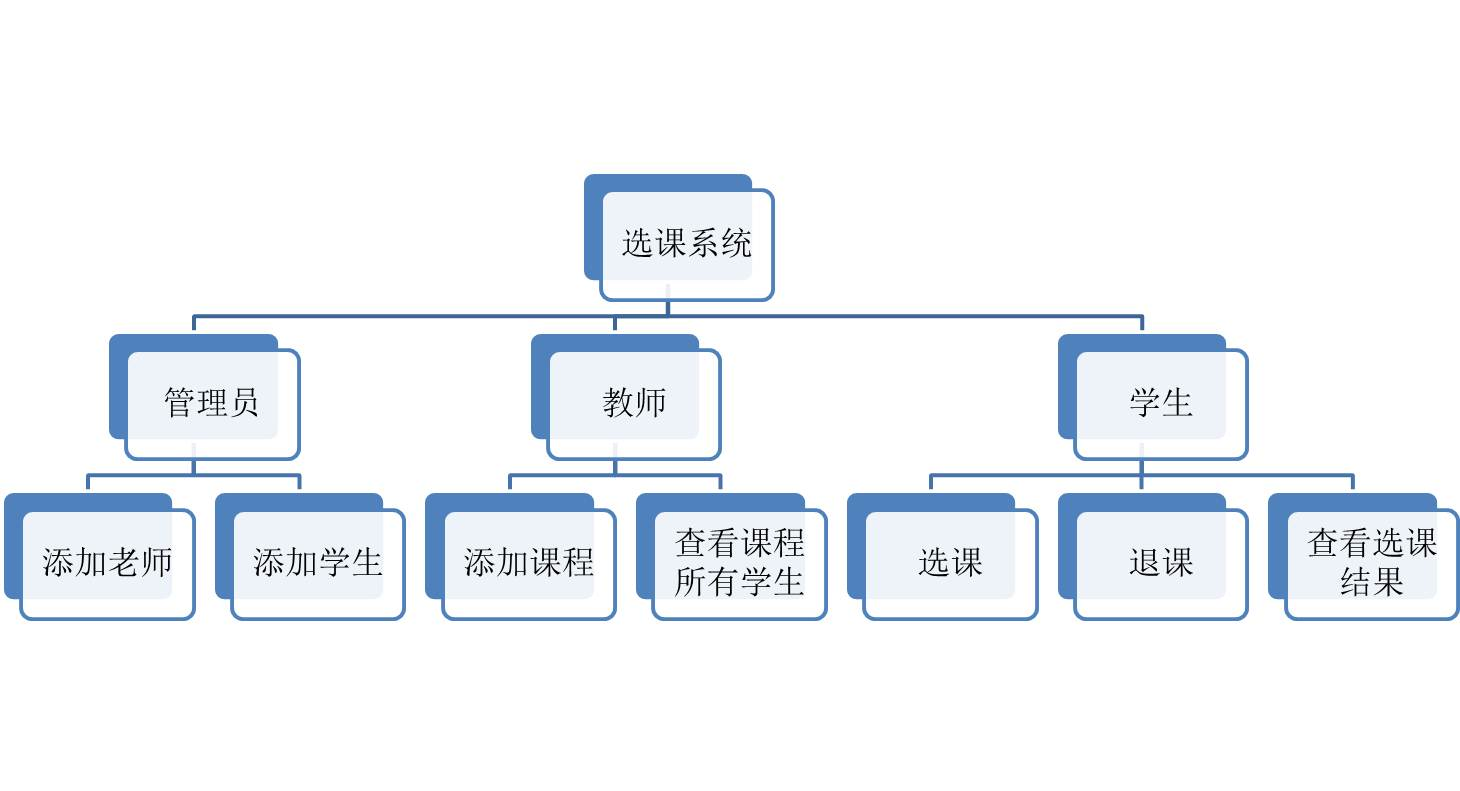
\includegraphics[scale=0.45]{S1.jpg}
\end{figure}

对于管理员、教师、学生、课程,分别创建类。

添加教师、学生、课程:直接在对应类上添加即可。

查看选中该课程的所有学生:遍历一次该课程的学生名单即可。

选课和退课:在相应课程中加入该学生或者删除该学生。

查看选课结果:暴力搜索所有课程,将所有该学生的课程显示出来。

\section{对象设计}

\begin{lstlisting}[language=C++]
//student.h

struct student {
    int stu_id;
    std::string name;
    student(int stu_id = 0, std::string name="") : stu_id(stu_id), name(name) {}
};

class student_list {
public:
    void init(); //read from hard disk
    void add();  //read from keyboard
    std::string id2name(int id); //convert id into name
    void write(); //write data into hard disk
private:
    std::vector <student> stu;
};
\end{lstlisting}

\begin{lstlisting}[language=C++]
//teacher.h

struct teacher {
    int tea_id;
    std::string name;
    student(int tea_id = 0, std::string name="") : tea_id(tea_id), name(name) {}
};

class teacher_list {
public:
    void init(); //read from hard disk
    void add();  //read from keyboard
    std::string id2name(int id); //convert id into name
    void write(); //write data into hard disk
private:
    std::vector <teacher> tea;
};
\end{lstlisting}

\newpage

\begin{lstlisting}[language=C++]
//course.h

struct course {
    int course_id;
    std::string name;
    int tea_id;
    std::vector<int> stu_id;
};

struct course_list {
public:
    void init();
    int add(std::string name, int tea_id);
    bool is_select(int course_id, int stu_id); //ask whether a student selected a course
    void select(int course_id, int stu_id); //do select process
    void unselect(int course_id, int stu_id); //do unselect process
    void write(); //write data into hard disk
    std::string get_all_course(); //show all course
    std::string get_course_info(int course_id); //show course info
private:
    std::vector<course> c;
};
\end{lstlisting}

\section{输入与输出}

使用标准输入输出与用户交互。

使用文件输入输出与硬盘数据交互:初始化时从硬盘读取数据,每完成一个操作,立即将修改写入文件。

\end{document}
















